\documentclass{article}

% Input packages & formatting
% Packages

% Math packages
\usepackage{amsmath} % Extended math functions
\usepackage{amssymb} % Extended math symbols (loads in amsfonts)
\usepackage{bm} % Bold math symbols
\usepackage{mathtools}

% Figure packages
\usepackage{caption} % Caption formatting for university standard
\usepackage{graphicx} % includegraphics command
\usepackage{subcaption} % Subfigures
\usepackage[section]{placeins} % Place floats in section
\usepackage{wrapfig}

% Table packages
\usepackage{booktabs} % Better tables
\usepackage{bigstrut} % Merged table cells
\usepackage{longtable} % Tables which overflow into next page
\usepackage{array}
\usepackage{colortbl} % Color table cells
\usepackage{makecell}
\usepackage{multirow}

% Fonts
\usepackage{lmodern} % Use latin modern rather than computer modern. Better for font encoding.
\usepackage[T1]{fontenc} % Allow text to be searchable in output

% Other packages
\usepackage{appendix} % Appendix environment
\usepackage{nextpage} % Cleartooddpage command
%\usepackage[square,comma,sort,numbers]{natbib} % Reference formatting
\usepackage{setspace} % Line spacing
\usepackage{listings} % Display code with syntax highlighting
\usepackage{upquote} % Vertical quotes in verbatim
\usepackage{xcolor} % Colors
\usepackage{titlesec} % Header spacing
\usepackage{xparse} % for tcolorbox
\usepackage[listings]{tcolorbox} % Colored boxes for highlighting syntax
\tcbuselibrary{breakable}
\tcbuselibrary{skins}
\usepackage{enumitem} % better enumerate/itemize options
\usepackage{fancyhdr}
\usepackage{multicol}
\usepackage{ifthen}
\usepackage{xstring}

% Table of contents
\usepackage{imakeidx} % Index page
\usepackage{tocloft} % Control of table of contents
\usepackage[nottoc]{tocbibind} % Adds bibliography, table of tables, table of figures, to table of contents
\usepackage[bookmarks,linktocpage,hidelinks]{hyperref} % Hyperlinks for sections, figures, etc.

% Bibliography
\usepackage[style=numeric]{biblatex}
\addbibresource{references/references.bib}
% Formatting
% Page format
\setlength{\oddsidemargin}{0.00in}  % Left side margin for odd numbered pages
\setlength{\evensidemargin}{0.00in} % Right side margin for even numbered pages
\setlength{\topmargin}{0.00in}      % Top margin
\setlength{\headheight}{0.20in}     % Header height
\setlength{\headsep}{0.20in}        % Separation between header and main text
\setlength{\topskip}{0.00in}        % Top skip
\setlength{\textwidth}{6.50in}      % Width of the text
\setlength{\textheight}{8.50in}     % Height of the text
\setlength{\footskip}{0.50in}       % Foot skip
\setlength{\parindent}{0.00in}      % First line indentation
\setlength{\parskip}{6pt}        % Space between two paragraphs

% Captions (figures, tables, etc.)
\setlength{\floatsep}{\parskip}          % Space left between floats.
\setlength{\textfloatsep}{\floatsep}   % Space between last top float
% or first bottom float and the text
\setlength{\intextsep}{\floatsep}      % Space left on top and bottom
% of an in-text float
\setlength{\abovecaptionskip}{0.1in plus 0.25in}  % Space above caption
\setlength{\belowcaptionskip}{0.1in plus 0.25in}  % Space below caption
\setlength{\captionmargin}{0.50in}     % Left/Right margin for caption
\setlength{\abovedisplayskip}{0.00in plus 0.25in} % Space before Math stuff
\setlength{\belowdisplayskip}{0.00in plus 0.25in} % Space after Math stuff
\setlength{\arraycolsep}{0.10in}       % Gap between columns of an array
\setlength{\jot}{0.10in}                % Gap between multiline equations
\setlength{\itemsep}{0.10in}           % Space between successive items

% Counters (no section numbering)
\setcounter{tocdepth}{3}
\setcounter{secnumdepth}{0}

% Spacing
\setstretch{1.5}

\titlespacing*{\section}{0cm}{6pt}{6pt}[0cm]
\titlespacing*{\subsection}{0cm}{6pt}{6pt}[0cm]
\titlespacing*{\subsubsection}{0cm}{6pt}{6pt}[0cm]

\titleformat{\section}
{\sffamily\huge}{}{0pt}{\titlerule\vspace{-0.2cm}}
\titleformat{\subsection}
{\sffamily\itshape\Large}{}{0pt}{}

% Macro for syntax
\newtcolorbox{syntax}{
    size=small,
    sharp corners,
    colframe=black,
    colback=yellow,
    fontupper=\bfseries\ttfamily
}

% Macro for argument table
\newenvironment{args}{
    \begin{tabular}{>{\bfseries\ttfamily}p{0.25\linewidth} p{0.69\linewidth}}
    }{
    \end{tabular}\par
    \vspace{0.5\baselineskip}
}

% Note: Requires packages "listing", "xcolor", and "textcomp"
\lstdefinelanguage{verbatim}{
    basicstyle=\ttfamily\small,
    xleftmargin=9pt,
    xrightmargin=9pt,
    columns=fullflexible,
    keepspaces=true,
    comment=[l]{\#},
    breaklines=true
}

\lstdefinestyle{verbatim}{
    commentstyle=\color{gray},
}

% Example code
\AtBeginDocument{
\newtcolorbox[blend into=listings]{example}[2][]{
    colback=blue!3!white,
    colframe=black,
    colbacktitle=blue!15!white,
    coltitle=black,
    sharp corners,
    enhanced,
    breakable,
    size=small,
    before upper={
        \setstretch{1.0}\lstset{language=verbatim,style=verbatim}\vspace{3pt}\textsf{\textit{Code:}}
    },
    subtitle style={
        colback=blue!20!white,
        fonttitle=\sffamily
    },
    before lower={
        \setstretch{1.0}\lstset{language=verbatim,style=verbatim}\vspace{3pt}\textsf{\textit{Output:}}
    },
    fonttitle=\sffamily,
    title={#2},
    #1
}
}


% Links to sub and subsub commands - optional boolean argument, default true. if false, only displays subcmd.

% Commands (and command ensembles)
\newcommand{\command}[1]{\protect\hypertarget{#1}{#1}\index{#1}}
\newcommand{\subcommand}[2]{\protect\hypertarget{#1 #2}{#1 #2}\index{#1!#2}}
\newcommand{\cmdlink}[1]{\protect\hyperlink{#1}{\textit{#1}}}
\newcommand{\subcmdlink}[3][1]{\protect\hyperlink{#2 #3}{\ifnum#1=1\relax\textit{#2 #3}\else\textit{#3}\fi}}

% Methods (first arg is class)
\newcommand{\method}[2]{\protect\hypertarget{$#1Obj #2}{\$#1Obj #2}\index{#1!#2}}
\newcommand{\methodlink}[3][1]{\protect\hyperlink{$#2Obj #3}{\ifnum#1=1\relax\textit{\$#2Obj #3}\else\textit{#3}\fi}}

% Macros for figure/table names
\newcommand{\fig}{\figurename\ }
\newcommand{\figs}{\figurename s }
\newcommand{\tbl}{\tablename\ }
\newcommand{\tbls}{\tablename s }
\newcommand{\eq}{Eq. }
\newcommand{\eqs}{Eqs. }
\renewcommand{\lstlistingname}{Example}% Listing -> Example
\renewcommand{\lstlistlistingname}{List of \lstlistingname s}% List of Listings -> List of Examples
\newcommand{\ex}{Example }
\newcommand{\exs}{Examples }
\newcommand{\var}[1]{\texttt{\textbf{\$#1}}}

% Header/footer
\renewcommand{\headrulewidth}{0pt}

\fancypagestyle{main}{
\fancyhf{}
\fancyhead[RE,LO]{\textsf{Object-Oriented Incremental Dynamic Analysis (ooida)}}
\fancyhead[LE,RO]{\textsf{\thepage}}
}

\fancypagestyle{chapter}{
\fancyhf{}
\fancyfoot[LE,RO]{\textsf{\thepage}}
}

\fancypagestyle{foreword}{
\fancyhf{}
\fancyfoot[C]{\textsf{\thepage}}
}

% Changes to hyperlinks (URLs)
\renewcommand\UrlFont{\color{blue}\rmfamily}

% New column type 
% https://tex.stackexchange.com/questions/75717/how-can-i-mix-itemize-and-tabular-environments
\newcolumntype{L}{>{\labelitemi~~}l<{}}
\newcommand{\version}{0.2}

\newcommand{\caret}{$^\wedge$}

% Figure path and type
\pdfminorversion=6
\DeclareGraphicsExtensions{.pdf,.png}
\graphicspath{{./figures/}}

% Other macros
\renewcommand{\^}[1]{\textsuperscript{#1}}
\renewcommand{\_}[1]{\textsubscript{#1}}

\title{\LARGE Object-Oriented Incremental Dynamic Analysis (ooida)\\\small Version \version}
\author{Alex Baker\\\small\url{https://github.com/ambaker1/ooida}}
\date{\small\today}
\makeindex[columns=1,title={Command Index}]
\begin{document}
\maketitle
\thispagestyle{empty}
\clearpage
\fancypagestyle{plain}[foreword]{}
\pagestyle{plain}
\clearpage
\pagenumbering{roman}
\tableofcontents
\markboth{}{}
\clearpage
\fancypagestyle{plain}[chapter]{}
\pagestyle{main}
\pagenumbering{arabic}
\section{General}
Incremental Dynamic Analysis (IDA) is a methodology for collapse assessment of buildings, and is essentially a parametric study, investigating the nonlinear response of a structure exposed to different earthquakes at increasing intensity. 
Of primary interest is to determine, at a high resolution, the collapse capacity of the structure for the given ground motion.
Of secondary interest is to trace the curve below the capacity point, to ensure that the capacity point is not part of a ``structural resurrection''.
The main hunt-fill tracing algorithm in this package is based on the original paper by Vamvatsikos and Cornell 2002 \cite{vamvatsikos_incremental_2002} and the parallel processing implementation is based on that described by Vamvatsikos and Cornell 2011 \cite{vamvatsikos_performing_2011}.

In similar fashion to the traditional hunt-fill tracing algorithm, the ``ooida'' package hunts for the capacity point and fills in the curve using a multi-staged approach:
\begin{enumerate}[label=\quad Stage \arabic*:,itemindent=*]
  \setcounter{enumi}{-1}
  \item Initialization stage, or simply the starting point. 
  \item ``Hunt-up'' stage, where it will increase the intensity until collapse is reached. 
  \item ``Bracketing'' stage, where it bisects to achieve desired precision on collapse capacity. 
  \item ``Fill-in'' stage, where the gaps below collapse are refined to achieve desired curve granularity. 
  \item Completion stage: collapse is reached and the curve is filled, but jobs may still be active.
\end{enumerate}

\subsection{Package Dependencies}
Due to the multi-stage nature of an IDA algorithm, and to facilitate running multiple IDA curves simultaneously, an Object-Oriented approach was adopted, using the standard ``TclOO'' package. 

Besides being able to run multiple IDA curves in parallel, intra-record parallelization (running multiple runs for a single curve simultaneously) is supported by the IDA algorithm for the ``fill-in'' stage, and implemented for OpenSeesMP using the ``mpjobs'' framework: \url{https://github.com/ambaker1/mpjobs}

As with the ``mpjobs'' framework, the ``ooida'' package utilizes the tabular data structure provided by the ``Tda'' package:
\url{https://github.com/ambaker1/Tda}.

All package dependencies are automatically installed if ``ooida'' is installed with the ``Tin'' package: \\\url{https://github.com/ambaker1/Tin}.

\clearpage
\section{Creating IDA Objects}
IDA objects are created from the \cmdlink{ida} class using the standard methods \textit{new} or \textit{create}.
Both class methods require definition of IDA settings \texttt{-collapse} and \texttt{-precision}. 
Once created, \cmdlink{ida} objects act as commands with an ensemble of subcommands, or methods. 
These objects can be copied with the method \methodlink[0]{ida}{copy} and deleted with the method \methodlink[0]{ida}{destroy}.
\begin{syntax}
\command{ida} new \$option \$value ... \\
ida create \$objectName \$option \$value ...
\end{syntax}
\begin{args}
\$objectName & Explicit name for object. \\
\$option \$value ... & Paired list of IDA options and corresponding values, see \methodlink{ida}{configure}.
\end{args}
\begin{example}{Creating an IDA object}
\begin{lstlisting}
set settings {}
dict set settings -huntup {Geometric 1.0 2.0}
dict set settings -collapse {SC {code != 0} NSC {drift > 0.10}}
dict set settings -precision {0.01 0.1}
set idaObj [ida new {*}$settings]
\end{lstlisting}
\end{example}

\subsection{Copying IDA Objects}
The method \methodlink[0]{ida}{copy} copies all the data from an IDA object to a new object.
\begin{syntax}
\method{ida}{copy} <\$objectName>
\end{syntax}
\begin{args}
\$objectName & Explicit name for object. By default, returns an auto-generated name.
\end{args}
\subsection{Removing IDA Objects}
The standard method \methodlink[0]{ida}{destroy} removes an IDA object from the interpreter. 
\begin{syntax}
\method{ida}{destroy}
\end{syntax}

\clearpage
\section{IDA Configuration}
The settings of an IDA object can be queried and modified with the method \methodlink[0]{ida}{configure}.
If this method is called with no arguments, it returns a dictionary of all configuration settings. 
If called with a single argument, it will return the current configuration for the specified setting. 
If called with more than one argument, the input will be parsed as a paired list of settings and configuration values to apply.
\begin{syntax}
\method{ida}{configure} \\
\$idaObj configure \$option \\
\$idaObj configure \$option \$value ...
\end{syntax}
\begin{args}
\$option ... & Setting options to set or query. \\
\$value ... & Configuration values for settings.
\end{args}
\FloatBarrier

\subsection{Collapse Criteria}
The collapse criteria must be defined with the \textit{-collapse} configuration setting. 
\begin{syntax}
-collapse "\$name1 \$cc1 \$name2 \$cc2 ... "
\end{syntax}
\begin{args}
\$name1 \$name2 ... & Unique collapse names. \\
\$cc1 \$cc2 ... & List of collapse criteria (\texttt{\$dm \$op \$value}), as described below: \\
\quad \$dm & \quad Damage measure name. \\
\quad \$op & \quad Comparison operator (\texttt{==} \texttt{!=} \texttt{>} \texttt{<} \texttt{>=} \texttt{<=} \texttt{in} \texttt{ni} \texttt{eq} or \texttt{ne}). \\
\quad \$value & \quad Value to compare to.
\end{args}
There are two types of collapse conditions: damage measure based and intensity measure based \cite{vamvatsikos_incremental_2002}. 
A damage measure based rule states that the first IDA point that exceeds the damage measure limit is the collapse point. 
An intensity measure based rule, on the other-hand, defines the collapse point as the last point with a slope greater than the limit. 
For example, FEMA report 350 defines the last point at which the tangent slope is greater than 20\% of the elastic IDA slope as the collapse point \cite{fema_recommended_2000}. 
Currently, the ``ooida'' package only supports damage-measure based rules.
\clearpage
\subsection{Hunt-up Method}
The algorithm used to determine the next intensity measure prior to collapse is defined with the \textit{-huntup} configuration setting.
If not specified, it will default to ``Geometric 1.0 2.0''.
\begin{syntax}
-huntup "\$type \$start \$step"
\end{syntax}
\begin{args}
\$type & Hunt-up method (\textit{Geometric}, \textit{Quadratic}, or \textit{Linear}, default \textit{Geometric}) \\
\$start & Starting intensity measure. Also starting step for \textit{Quadratic}. Default 1.0. \\
\$step & For \textit{Geometric}, the geometric ratio. For \textit{Quadratic}, the step increase. For \textit{Linear}, the step size. Default 2.0.
\end{args}
The \textit{Geometric} method ensures that the ratio between gaps is constant, while the \textit{Quadratic} method ensures that the difference between gaps is constant. To illustrate their differences, the hunt-up of a simple IDA curve $(\text{DM} = \text{IM}^2)$ is performed with both methods with the same number of steps and the same start and end point, as shown in \fig\ref{fig:ida_huntup}.

As can be seen in the figure, the \textit{Geometric} method can increase gap size more quickly, while the \textit{Quadratic} method produces more consistent gap sizes. In fact, if the \textit{Quadratic} ``step'' is set to 0.0, the gap sizes will be constant.
\begin{figure}[!htb]
\centering
\begin{subfigure}[b]{0.45\linewidth}
    \centering
    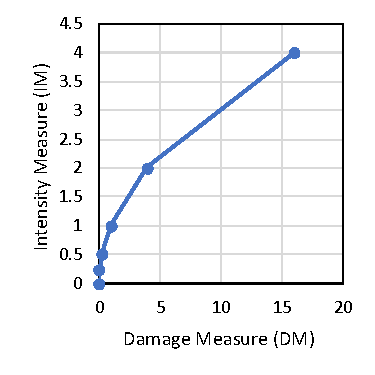
\includegraphics[width=2.5in]{ida_geometric_huntup}
    \caption{Geometric Hunt-up: \newline Start = 0.25, Step = 2.0}
    \label{fig:ida_geometric_huntup}
\end{subfigure}
\begin{subfigure}[b]{0.45\linewidth}
    \centering
    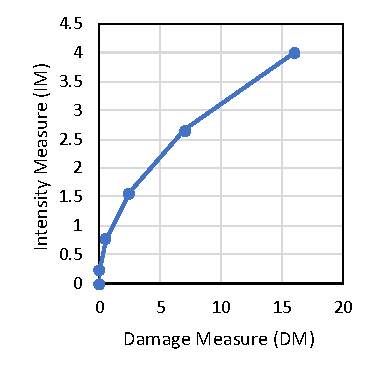
\includegraphics[width=2.5in]{ida_quadratic_huntup}
    \caption{Quadratic Hunt-up: \newline Start = 0.25, Step = 0.275}
    \label{fig:ida_quadratic_huntup}
\end{subfigure}
\caption{Geometric vs Quadratic Hunt-up}
\label{fig:ida_huntup}
\end{figure}
\clearpage
\subsection{Hunt and Fill Precision}
Once collapse is reached in the IDA algorithm, the algorithm will focus first on meeting precision on the capacity point, then on meeting precision on the rest of the IDA curve. 
For the hunt precision, the gap between the estimated capacity and the minimum collapse intensity is bisected until the gap is less than the tolerance.
For the fill precision, the gaps below the estimated capacity are bisected or trisected, going in order of largest gaps first, until no gap exists that is greater than the precision.
When both precision tolerances are met and all jobs are complete, the IDA curve is considered to be complete. 
\begin{syntax}
-precision "\$hunt \$fill"
\end{syntax}
\begin{args}
\$hunt & Intensity measure hunt precision. \\
\$fill & Intensity measure fill precision.
\end{args}
\clearpage
\subsection{IDA Curve Refining Limits}
Sometimes, the only information needed from an IDA is whether the capacity is above or below a certain value. 
In this case, the option \textit{-limits} can be used.
The -limits option define upper and lower intensity measure limits for collapse refining. 
By default, they are set to 0 and Inf, respectively. 
\begin{syntax}
-limits "\$lower \$upper"
\end{syntax}
\begin{args}
\$lower & Lower limit for refining collapse point. \\
\$upper & Upper limit for refining collapse point.
\end{args}

The limits define three intensity measure zones as shown in \fig\ref{fig:ida_zones}. 
In the figure, if collapse has not been reached, the minimum collapse can be considered to be in zone 3. \\

\begin{figure}[!htb]
\centering
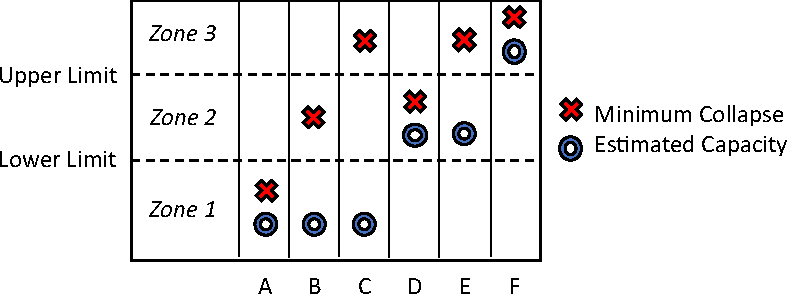
\includegraphics{ida_zones}
\caption{Partial IDA Zones}
\label{fig:ida_zones}
\end{figure}

Depending on which zones the the capacity and minimum collapse points are, it will modify the behavior of the IDA as described below:

\begin{tabular}{cp{0.9\linewidth}}
A & Both estimated capacity and minimum collapse are in zone 1. No more runs are required. \\
B & Capacity is below lower limit, but minimum collapse is above. Fill-in stage is not needed. \\
C & Same as B.\\
D & Both estimated capacity and minimum collapse are in zone 2. Full refinement is necessary to capture any structural resurrections. \\
E & Same as D. \\
F & Both estimated capacity and minimum collapse are in zone 3. Hunting and bracketing are not required, but curve must be filled in below upper limit to capture any structural resurrections.
\end{tabular}
%In general, if the capacity is below the lower limit, it will not refine the curve further, and if the capacity is above the maximum, the curve will only be filled in below the upper limit, to capture any potential structural resurrections that could change the relative capacity. 
%More specifically, there are six potential configurations that are handled by the \textit{-limit} option, described below:



\clearpage
\section{Running an IDA}
The ``ooida'' package does not run the individual dynamic analyses of an IDA.
Rather, it provides a guiding framework for tracing IDA curves. 
Individual runs are run either directly in the current instance of OpenSees, or with a job using the job board framework (recommended due to its save-state functionality).
\subsection{Adding IDA Points}
IDA data points are inputted via the method \methodlink[0]{ida}{add}. 
If the input is a single item, it is interpreted as a job name, using the job board framework.
If the job is posted but not running, it will run the job.
If the input is a key-value paired list, it is interpreted as damage measure names and values.
The only reserved keys are ``collapsed'', ``intensity'', and ``jobTag''.
\begin{syntax}
\method{ida}{add} \$im <\$jobTag> <\$dmName \$dmValue ...>
\end{syntax}
\begin{args}
\$im & Intensity measure to add. \\
\$jobTag & Integer job tag, using the job board framework, that corresponds to the intensity measure.  \\
\$dmName \$dmValue ... & Paired list of damage measure names and values for the intensity measure. Mutually exclusive with \$jobTag.
\end{args}

\subsection{Removing IDA Points}
The method \methodlink[0]{ida}{remove} removes an intensity measure from an IDA curve.
If the intensity measure does not exist in the IDA object, it will do nothing.
\begin{syntax}
\method{ida}{remove} \$im
\end{syntax}
\begin{args}
\$im & Intensity measure to remove.
\end{args}
\clearpage
\subsection{Wiping the IDA}
An IDA can be wiped with the method \methodlink[0]{ida}{wipe}.
This removes all existing points and resets collapse information, but maintains any IDA configuration settings.
\begin{syntax}
\method{ida}{wipe}
\end{syntax}

\subsection{Getting the Next Intensity Measure}
The next intensity measure to run according to the hunt-up settings, collapse criteria, and precision values, can be queried with \methodlink{ida}{next}. 
Returns -1 if waiting on active jobs, and -2 if all criteria are met. 
\begin{syntax}
\method{ida}{next}
\end{syntax}

\subsection{Check if IDA is Complete}
The completion status of an IDA curve can be queried with \methodlink{ida}{complete}. 
The IDA is considered complete when collapse is reached, hunt and fill precisions are met, and no active jobs remain.
This is equivalent to checking if the next intensity is -2.
\begin{syntax}
\method{ida}{complete}
\end{syntax}

\subsection{Updating the IDA}
If using the job board framework for running an IDA, results from jobs will only be added when \methodlink[0]{ida}{update} is called. 
This method is automatically called during  \methodlink[1]{ida}{run}.
\begin{syntax}
\method{ida}{update}
\end{syntax}
\clearpage
\subsection{Run an IDA}
For convenience, the flow of an IDA can be controlled entirely with \methodlink{ida}{run}.
\begin{syntax}
\method{ida}{run} \$imVar \$body
\end{syntax}
\begin{args}
\$imVar & Variable to pass next intensity measure to. \\
\$body & Body to evaluate that runs each IDA point. Must evaluate to a result dictionary or a job tag, in the same fashion as the Tcl command ``lmap''.
\end{args}

\begin{example}{Running a single IDA in series}
\begin{lstlisting}
$ida run Sa {
    wipe
    source DoDynamic.tcl
}
\end{lstlisting}
\end{example}
\begin{example}{Running a single IDA with ``mpjobs'' framework (series or parallel)}
\begin{lstlisting}
jobBoard IDA {
    $ida run Sa {
    	makeJob DoDynamic.tcl Sa $Sa
    }
}
\end{lstlisting}
\end{example}

\clearpage
\section{Getting IDA State Information}
Various methods are provided for accessing the state of the IDA.
\subsection{IDA Stage}
The stage of the IDA can be queried with the method \methodlink[0]{ida}{stage}.
\begin{syntax}
\method{ida}{stage}
\end{syntax}
\subsection{Estimated Capacity}
The estimated capacity, as in the largest intensity measure value below the minimum collapse, can be queried with the method \methodlink[0]{ida}{capacity}.
\begin{syntax}
\method{ida}{capacity}
\end{syntax}
\subsection{Whether Collapse Was Reached}
The method \methodlink[0]{ida}{collapsed} returns 1 if collapse was reached, and zero otherwise.
\begin{syntax}
\method{ida}{collapsed}
\end{syntax}
\subsection{Minimum Collapse}
The minimum collapse intensity, if collapse was reached, can be queried with the method \methodlink[0]{ida}{minCollapse}.
If collapse was not reached, it will return blank.
\begin{syntax}
\method{ida}{minCollapse} <\$name>
\end{syntax}
\begin{args}
\$name & Collapse name associated with collapse criteria. Default returns minimum for all collapse criteria.
\end{args}
\clearpage
\subsection{List of All Intensities}
A sorted list of all intensity measure values can be queried with \methodlink{ida}{getIMs}.
\begin{syntax}
\method{ida}{getIMs}
\end{syntax}
\subsection{Damage Measure Curve}
A damage measure curve, in matrix form, can be queried with \methodlink{ida}{curve}.
The first column of the matrix will be the damage measure values, and the second column will be the intensity values, in increasing order.
\begin{syntax}
\method{ida}{curve} \$dm
\end{syntax}
\begin{args}
\$dm & Damage measure name.
\end{args}
\subsection{Estimated Empirical CDF}
If the IDA object is a part of a suite object, the method \methodlink[0]{ida}{cdf} will return the estimated CDF for the corresponding ground motion. 
Otherwise, the method does not exist.
\begin{syntax}
\method{ida}{cdf}
\end{syntax}

\subsection{Getting Table of IDA Data}
The method \methodlink[0]{ida}{table} returns a ``Tda'' table object containing IDA curve data, where keys correspond to intensity measure values and fields correspond to damage measures. 
Additionally, the table includes a field called ``jobTag'', a field named ``collapsed'', which is 1 if the intensity is above capacity, and 0 otherwise, and fields for each collapse criteria name.

\begin{syntax}
\method{ida}{table}
\end{syntax}
The IDA curve can be easily exported to CSV with the ``Tda'' command \textit{writeTable}, as shown below.
\begin{example}{Exporting IDA table to CSV}
\begin{lstlisting}
writeTable curve.csv [$idaObj table]
\end{lstlisting}
\end{example}

\clearpage
\section{IDA Suite Objects}
Since IDAs are typically done with a suite of ground motions, an wrapper class is provided: \cmdlink{suite}.
This wrapper class can be used to easily run multiple IDAs simultaneously.
Suite objects, like IDA objects, are created from the \cmdlink{suite} class using the standard methods \textit{new} or \textit{create}.
Once created, \cmdlink{suite} objects act as commands with an ensemble of subcommands, or methods, and can be deleted with the method \methodlink[0]{suite}{destroy}.
\begin{syntax}
\command{suite} new <-medianSearch \$medianSearch> \\
suite create \$objectName <-medianSearch \$medianSearch>
\end{syntax}
\begin{args}
\$objectName & Explicit name for object. \\
\$medianSearch & Whether to do partial IDA, targeting median CDF. Default false.
\end{args}

The \textit{-medianSearch} option toggles the partial IDA refinement algorithm, which minimizes the number of analyses required to obtain the median collapse intensity measure required for FEMA P-695 analyses \cite{fema_quantification_2009}. 
Further explanation of the partial IDA refinement algorithm can be found in \cite{baker_kinematics_2022}.  

\subsection{Removing Suite Objects}
The standard method \methodlink[0]{suite}{destroy} removes an IDA suite object from the interpreter, and also destroys any linked IDA objects.
\begin{syntax}
\method{suite}{destroy}
\end{syntax}
\clearpage

\subsection{Adding IDA Objects to Suite}
The method \methodlink[0]{suite}{add} adds an IDA curve to the suite.
Adding an IDA to a suite sets up a ``write'' trace on the capacity variable of the IDA object, such that whenever it changes, the estimated fragility curve is updated accordingly.
Additionally, if the \textit{-medianSearch} option is set, it will then update the \textit{-limits} configuration of each IDA object to reduce the number of extraneous runs.
It also adds the \methodlink[0]{ida}{cdf} method to the IDA object.
\begin{syntax}
\method{suite}{add} \$gm \$idaObj
\end{syntax}
\begin{args}
\$gm & Ground motion name to identify IDA by. \\
\$idaObj & IDA object.
\end{args}
\subsection{Removing IDA Objects from Suite}
The method \methodlink[0]{suite}{remove} removes an IDA curve from the suite.
It also removes the associated variable trace and \methodlink[0]{ida}{cdf} method from the IDA object.
\begin{syntax}
\method{suite}{remove} \$gm
\end{syntax}
\begin{args}
\$gm & Ground motion name to identify IDA by.
\end{args}

\subsection{Getting the Next Ground Motion and Intensity}
Similar to \methodlink{ida}{next}, the next ground motion and intensity measure can be queried with \methodlink{suite}{next}.
If waiting on active jobs, it will return ``\texttt{\{\} -1}'', and if all ground motions are complete, it will return ``\texttt{\{\} -2}''. 
Otherwise, it will return a list of the ground motion and an intensity measure to run. 
If called multiple times, it will cycle through the available IDA curves.
\begin{syntax}
\method{suite}{next}
\end{syntax}
\clearpage
\subsection{Checking if all IDA are Complete}
The method \methodlink[0]{suite}{complete} returns 1 if all IDA curves are complete, and 0 otherwise.
\begin{syntax}
\method{suite}{complete}
\end{syntax}

\subsection{Updating an IDA Suite}
If using the job board framework for running an IDA suite, results from jobs will only be added when \methodlink{ida}{update} is called for each IDA.
The suite method \methodlink[0]{suite}{update} simply calls the corresponding IDA method for each IDA object in the suite.
This method is automatically called during  \methodlink{suite}{run}.
\begin{syntax}
\method{suite}{update}
\end{syntax}

\subsection{Running an IDA Suite}
For convenience, the flow of running an entire IDA suite can be controlled entirely with \methodlink{suite}{run}.
\begin{syntax}
\method{suite}{run} \$gmVar \$imVar \$body
\end{syntax}
\begin{args}
\$gmVar & Variable to pass next ground motion to. \\
\$imVar & Variable to pass next intensity measure to. \\
\$body & Body to evaluate that runs each IDA point. Must evaluate to a result dictionary or a job tag, in the same fashion as the Tcl command ``lmap''.
\end{args}

\begin{example}{Running an IDA suite in series}
\begin{lstlisting}
$suite run gmFile Sa {
    wipe
    source DoDynamic.tcl
}
\end{lstlisting}
\end{example}
\begin{example}{Running an IDA suite with ``mpjobs'' framework (series or parallel)}
\begin{lstlisting}
$suite run gmFile Sa {
    makeJob DoDynamic.tcl gmFile $gmFile Sa $Sa
}
\end{lstlisting}
\end{example}
\clearpage
\subsection{Accessing Suite IDA Objects}
The IDA objects in a suite can be queried or called directly with \methodlink{suite}{ida}.
\begin{syntax}
\method{suite}{ida} \$gm \$arg1 \$arg2 ...
\end{syntax}
\begin{args}
\$gm & Ground motion associated with IDA object. \\
\$arg1 \$arg2 ... & Arguments to pass to IDA object. If none, it will return the IDA object.
\end{args}

\subsection{Getting all Ground Motions in Suite}
The method \methodlink[0]{suite}{getGMs} returns a list of all ground motions defined for the suite.
\begin{syntax}
\method{suite}{getGMs}
\end{syntax}

\subsection{Getting Summary Table of Fragility Data}
The method \methodlink[0]{suite}{table} returns a ``Tda'' table, where the ground motions are the keys and sorted in increasing collapse capacity.
The fields in the fragility data table are as follows:

\begin{tabular}{ll}
\toprule
Field & Description \\
\midrule
capacity & Collapse intensity (result of \methodlink[1]{ida}{capacity}). \\
cdf & Cumulative distribution function (CDF) value of fragility curve. \\
collapsed & Whether the ground motion reached collapse. \\
... & Collapse criteria names defined with -collapse option of \methodlink[1]{ida}{configure}.\\
\bottomrule
\end{tabular}


\begin{syntax}
\method{suite}{table}
\end{syntax}
The fragility data can be easily exported to CSV with the ``Tda'' command \textit{writeTable}, as shown below.

\begin{example}{Using ``Tda'' table methods to access fragility data}
\begin{lstlisting}
set fragilityData [$suiteObj table]
set gms [$fragilityData keys]; # list of ground motions, in order of increasing collapse capacity
set cdf [$fragilityData cget cdf]; # List of cdf values for each ground motion
writeTable fragility.csv $fragilityData
\end{lstlisting}
\end{example}

\clearpage	
\section{Example Applications}
The ``ooida'' package is a flexible framework for running incremental dynamic analyses.
It can be used to process existing data, trace IDA curves in series, or trace IDA curves in parallel using the job board framework.
\subsection{Process Existing Data}
Since the IDA framework does not actually run the analyses, existing data can be added directly to an IDA object.
\begin{example}{Add existing data from CSV file with intensity as first column}
\begin{lstlisting}
package require tin
tin import readTable from tda
set idaTable [readTable idadata.csv]; # from ida table output
dict for {im results} [$idaTable data] {
    $idaObj add $im {*}$results
}
\end{lstlisting}
\end{example}
\subsection{Tracing an IDA Curve in Series}
The job board framework is not needed for running an IDA in series, as shown in the example below.
\begin{example}{IDA of a nonlinear frame (RunDynamic.tcl) in series}
\begin{lstlisting}
package require tin
tin import writeTable from tda
# Series example
set idaObj [ida new -huntup {Geometric 0.1 2.0} -collapse {NSC {drift > 0.10}} \
        -precision {0.005 0.01}]
$idaObj run Sa {
    wipe 
    source RunDynamic.tcl
}
# Save data to file
writeTable idadata.csv [$idaObj table]
\end{lstlisting}
\end{example}
\clearpage
\subsection{Tracing Multiple IDA Curves in Parallel}
Using the ``ooida'' package and the ``mpjobs'' package, it is easy to run multiple IDA curves in parallel, with load sharing between curves, as shown in the example below. 

\begin{example}{IDA for suite of ground motions in parallel}
\begin{lstlisting}
# Main loop (load shares between IDA curves!)
package require tin
tin import writeTable from tda
tin import mpjobs
tin import ooida
jobBoard -wipe IDA {
    # Create suite object
    set settings ""
    dict set settings -huntup {Geometric 0.1 2.0}
    dict set settings -collapse {NSC {drift > 0.10}}
    dict set settings -precision {0.005 0.01}
    set suite [suite new]
    foreach gmFile [glob -directory GMs *.AT2] {
        $suite add $gmFile [ida new {*}$settings]
    }

    $suite run gmFile Sa {
        makeJob RunDynamic.tcl gmFile $gmFile Sa $Sa
    }

    # Export data
    writeTable fragility.csv [$suite table]
    foreach gmFile [$suite getGMs] {
        set gmName [file rootname [file tail $gmFile]]
        writeTable $gmName.csv [$suite ida $gmFile table]
    }
}
\end{lstlisting}
\end{example}

\phantomsection
\interlinepenalty=1000
\printbibliography[heading=bibintoc]
\printindex
\end{document}
